%Đây là template dùng cho đề cương đề tài tốt nghiệp
%Khoa Công nghệ Thông tin
%Trường Đại học Khoa học Tự nhiên, ĐHQG-HCM

%Liên hệ về mẫu LaTEX này: Thầy Bùi Huy Thông (bhthong@fit.hcmus.edu.vn)

\documentclass{article}[14pt]
\usepackage[utf8]{vietnam}
\usepackage{enumerate}
\usepackage{enumitem}
\usepackage{multicol}
\usepackage{listings}
\usepackage[left=2cm,right=2cm,top=2.5cm,bottom=2.5cm]{geometry}
\usepackage{verbatim}
\usepackage{graphicx}
\usepackage{url}
\usepackage{fancyhdr}
\usepackage{fancybox,framed}
\linespread{1.3}
\usepackage{lastpage}
\usepackage{floatrow}
\usepackage{floatrow}
\usepackage{caption}
\pagenumbering{arabic}
%\pagestyle{fancy}
\newfloatcommand{capbtabbox}{table}[][\FBwidth]

\usepackage{blindtext}
\usepackage{titlesec}
\usepackage[nottoc]{tocbibind}

\titleformat*{\section}{\LARGE\bfseries}
\titleformat*{\subsection}{\Large\bfseries}
\titleformat*{\subsubsection}{\large\bfseries}
%\addbibresource{ref.bib}


\begin{document}
    \begin{figure}[h]
        \begin{floatrow}
        \ffigbox{
\includegraphics[scale = .4]{logo.png}}  
        {%
    
        }
        \capbtabbox{
            \begin{tabular}{l}
            \multicolumn{1}{c}{\textbf{\begin{tabular}[c]{@{}c@{}}TRƯỜNG ĐẠI HỌC KHOA HỌC TỰ NHIÊN\\KHOA CÔNG NGHỆ THÔNG TIN\end{tabular}}} \\ \\ \\
            \end{tabular}
        }
        {%
    
        }
        \end{floatrow}
    \end{figure}
    
    \begin{center}
        
        %Xác định loại đề tài tốt nghiệp tương ứng: Khóa luận, Thực tập, Đồ án
        \textbf{\Large ĐỀ CƯƠNG KHOÁ LUẬN TỐT NGHIỆP} \\ 
    \end{center}
    
    %\vspace{.5cm}
    
    \begin{center}
    %Tên đề tài phải VIẾT HOA
        
        \textbf{\huge HỌC TỰ GIÁM SÁT TRÊN MẠNG HỌC SÂU ĐỒ THỊ CHO HỆ THỐNG GỢI Ý} 
        \\
        
    %Tên đề tài bằng tiếng Anh (nếu có)
    \vspace{.5cm}
        \textit{\textbf{\Large (Self-supervised Graph Learning for Recommendation)}}
    \end{center}
    
    \vspace{.5cm}
    
    \Large
    \section{THÔNG TIN CHUNG}
    \begin{itemize}[label = {}]
        
        \item \textbf{Người hướng dẫn:} 
        %Thể hiện dạng: <Chức danh> <Họ và tên> (<Đơn vị công tác>)
        \begin{itemize}
            \item GS. TS. Lê Hoài Bắc  (Khoa Công nghệ thông tin)
        \end{itemize}{}
    
        
        \item \textbf{Nhóm sinh viên thực hiện:}
        
        %Thể hiện dạng: <Họ và tên sinh viên> (MSSV: )
        \begin{enumerate}
        
            \item Hồ Trần Việt Cường (MSSV: 19120056) 
            \item Nguyễn Trung Dũng (MSSV: 19120486)
        \end{enumerate}

       %Chọn loại thích hợp
        \item \textbf{Loại đề tài:} Nghiên cứu
        
        \item \textbf{Thời gian thực hiện:} Từ \textit{1/2023} đến \textit{6/2023}
        
        
    \end{itemize}
    
    \pagebreak 
    
    \section{NỘI DUNG THỰC HIỆN}

    %Mỗi mục dưới đây phải viết ít nhất là 5 câu mô tả/giới thiệu.
    
    \subsection{Giới thiệu về đề tài}
    
    Bài toán hệ thống gợi ý là một dạng bài xây dựng một hệ thống với khả năng hỗ trợ ra quyết định, cung cấp các gợi ý cho người dùng về những “sản phẩm” mà họ có thể cần. Với những “sản phẩm" đúng, ta có thể mang lại trải nghiệm tốt cho người dùng, xa hơn là có thể thúc đẩy phát triển kinh doanh.

    Vậy đầu vào, đầu ra của bài toán này là gì? Ở đầu vào, ta cần đưa cho hệ thống gợi ý lịch sử tương tác với “sản phẩm” của một hoặc nhiều người dùng. Đầu ra của hệ thống sẽ dự đoán về hành vi, “sản phẩm” của người dùng có thể thích hay cần ở hiện tại hoặc tương lai.
    
    Tuy nhiên, bài toán hệ thống gợi ý đang phải giải quyết một số vấn đề \cite{issues}:
    \begin{itemize}[leftmargin=10mm]
        \item Dữ liệu thưa:
            \begin{itemize}
                \item Dữ liệu thưa hiểu nôm na là dữ liệu có rất nhiều giá trị bằng 0/null (khác với dữ liệu bị thiếu).
                \item Trong ngữ cảnh của hệ thống gợi ý, người dùng có khuynh hướng chỉ tương tác với một phần rất nhỏ trong cơ sở dữ liệu của hàng triệu các “sản phẩm”, các tương tác này có thể được coi như là dữ liệu có giá trị khác 0/null và các tương tác không tồn tại với các “sản phẩm” khác sẽ được coi như là có giá trị 0/null. Vậy nên việc tìm ra nhiều người dùng mà có lịch sử tương tác giống nhau, hay việc phân tích tương tác của người dùng đối với một tập “sản phẩm” nhất định là rất khó.
                \item Vì sự khó khăn về việc tìm hành vi giống nhau của người dùng và phân tích hành vi nên dữ liệu thưa là một vấn đề lớn để đưa ra dự đoán về tương tác của người dùng một cách đáng tin cậy. Đối với hệ thống gợi ý thì hiệu năng của nó bị ảnh hưởng một cách đáng kể.
            \end{itemize}
        \item Sự thay đổi hành vi người dùng:
            \begin{itemize}
                \item Sở thích và hành vi của người dùng không cố định và thường thay đổi rất nhanh theo thời gian và tùy vào nhiều trường hợp và các yếu tố khác nhau.
                \item Rating của người dùng chỉ mang tính nhất thời tại một thời điểm và bị nhiều yếu tố tác động.
            \end{itemize}
        \item Vấn đề về riêng tư của người dùng:
            \begin{itemize}
                \item Để có thể đưa ra các gợi ý phù hợp cho người dùng, hệ thống gợi ý cần khá nhiều thông tin về sở thích và lịch sử tương tác của họ. Có thể nói dữ liệu này rất nhạy cảm và mang nhiều rủi ro, có giá trị rất lớn và dễ là đối tượng cho tin tặc tấn công, hoặc bị bán cho các công ty quảng cáo…
                \item Trong khi đó, đa số người dùng thường không biết lượng thông tin mà họ cung cấp cho các hệ thống này lớn tới đâu, và không biết thông tin đó đang được dùng để làm gì.
            \end{itemize}
    \end{itemize}

    Bài toán xây dựng hệ thống gợi ý là bài toán không mới, tuy nhiên nó cũng chỉ mới “nở rộ" cách đây không lâu \cite{soa}, và cũng còn rất nhiều tiềm năng để phát triển. Học giám sát (Supervised Learning) cần một lượng lớn dữ liệu được gán nhãn cẩn thận. Việc này đòi hỏi một lượng thời gian lớn và rất tốn kém, trong khi đó lượng dữ liệu chưa được gán nhãn thì lại rất nhiều và liên tục được sinh ra. Gần đây, có một hướng nghiên cứu có thể giải quyết được việc này, bằng cách học chính những đặc trưng bên trong của dữ liệu chưa được gán nhãn là \textbf{học tự giám sát (Self-supervised Learning)}. Hướng nghiên cứu đó còn mới, việc áp dụng mô hình học đó vào bài toán hệ thống gợi ý lại càng mới hơn. Chính vì vậy, nhóm em sẽ chọn hướng tiếp cận đó để nghiên cứu.
    
    %\textbf{Ghi chú:} Cần đăng ký tài khoản trên Overleaf\footnote{https://www.overleaf.com} và đọc cách sử dụng LaTeX tại hướng dẫn này \footnote{https://www.overleaf.com/learn/latex/Learn\_LaTeX\_in\_30\_minutes}% \cite{overleaf}.
    
    \subsection{Mục tiêu đề tài}
    
    %Phần này mô tả về động lực để giải quyết vấn đề.
    Tại sao cần thực hiện đề tài này?
    \begin{itemize}
        \item Như đã đề cập ở trên, hiện nay hệ thống gợi ý là một bài toán rất khó để cải tiến, ta thấy học tự giám sát là một phương pháp đáng hứa hẹn ở hiện tại và tương lai. Với đề tài này, ta sẽ biết được tình hình nghiên cứu về bài toán học tự giám sát trên mạng học sâu đồ thị cho hệ thống gợi ý trong thời gian gần đây. Qua đó biết được các hướng nghiên cứu đã và đang được hướng tới, vấn đề đã giải quyết được, ưu nhược điểm của các phương pháp và các vấn đề vẫn cần phải quyết trong tương lai.
    \end{itemize}
    Đề tài mang lại được điều gì?
    \begin{itemize}
        \item Hiểu rõ lý thuyết xoay quanh bài toán học giám sát trên mạng học sâu đồ thị cho hệ thống gợi ý (về mạng học sâu đồ thị, hệ thống gợi ý và học tự giám sát) một cách có hệ thống
        \item Có thể giải quyết được phần nào vấn đề mà hệ thống cũ còn tồn tại dựa trên học tự giám sát
    \end{itemize}
    Ảnh hưởng và ý nghĩa có thể có của kết quả đối với vấn đề đã được đặt ra nói riêng và toàn bộ hướng nghiên cứu nói chung?
    \begin{itemize}
        \item Việc này có thể giải quyết một phần nào đó các vấn đề mà các hướng nghiên cứu trước đang gặp phải (vấn đề dữ liệu thưa,...) Từ đó mở ra được các hướng nghiên cứu mới hơn, hiệu quả hơn trong bài toán hệ thống gợi ý.
    \end{itemize}
    \subsection{Phạm vi của đề tài}
    
    Nhóm em sẽ sử dụng 3 bộ dataset để tiến hành thí nghiệm:
    \begin{itemize}
        \item Yelp 2018: dataset của Yelp, chứa thông tin về doanh nghiệp, người dùng, và review của người dùng về các doanh nghiệp đó.
        \item Amazon Book: data review của người dùng từ Amazon trong khoảng từ năm 1996 đến 2014.
        \item Alibaba ifashion: dataset công khai của Alibaba, gồm các sản phẩm thời trang của trang bán hàng online và các tương tác của người dùng.
    \end{itemize}

    Đề tài sẽ tập trung về việc giải thích học tự giám trên mạng học sâu đồ thị được áp dụng vào hệ thống gợi ý. Bên cạnh đó nhóm sẽ tiến hành một số thí nghiệm nhằm cải tiến thêm dựa trên những vấn đề đang gặp phải của hệ thống bên trên nếu có thời gian.
    
    \subsection{Cách tiếp cận dự kiến}
    
    %Có thể bổ sung hình ảnh vào để làm rõ phương pháp hoặc cách tiếp cận dự kiến.
    Không giống như bài toán gắn nhãn cho ảnh, việc có được một bộ dữ liệu cho bài toán gợi ý cực kỳ tốn kém vì dữ liệu được tạo ra bởi chính bản thân người dùng, trong khi đó đa số người dùng chỉ tương tác với một phần nhỏ các mục/vật phẩm. Vì vậy, vấn đề về dữ liệu huấn luyện là một chướng ngại gây cản trở các model gợi ý học sâu có thể đạt được tiềm năng của nó. 

    Ngoài ra không phải lúc nào data cũng được gán nhãn sẵn. Trong nhiều trường hợp thực tế, ta phải đối mặt với với một lượng lớn data không được gán nhẵn. Với học tự giám sát, mô hình có thể học được từ những đặc trưng chính từ bên trong của dữ liệu từ đó cải thiện độ chính xác của mô hình.
    
    Hiện tại, với bài toán hệ thống gợi ý, ta có 3 hướng \cite{soa} chính tiếp cận như sau:
    \begin{itemize}[leftmargin=10mm]
        \item Content-based systems: xây dựng một profile dựa trên các item mà người dùng tương tác, từ đó dự đoán các item mới có khả năng thuộc về profile đó hay không.
        \item Collaborative filtering: dựa trên hành vi của nhiều người dùng lên một item để dự đoán mức độ quan tâm của người dùng lên sản phẩm dựa trên một độ đo giống nhau giữa các người dùng.
        \item Hybrid filtering: kết hợp Content-based và Collaborative filtering.
    \end{itemize}

    Tuy nhiên các cách tiếp cận trên vẫn chưa giải quyết được vấn đề dữ liệu thưa như đã nêu ở đầu giới thiệu đề tài.

    \textbf{Self-supervised Recommendation (SSR)} có tiềm năng giải quyết được vấn đề của hệ thống gợi ý.

    Các đặc trưng của Self-supervised Recommendation:
    \begin{itemize}[leftmargin=10mm]
        \item Thu được nhiều tín hiệu giám sát bằng việc bán tự động khai thác dữ liệu thô.
        \item Có một pretext task để pretrain các mô hình với dữ liệu được tăng cường. Điều này giúp phân biệt SSR với các phương pháp gợi ý khác.
        \item Với recommendation task đóng vai trò chính, pretext task đóng vai trò phụ nhằm tăng cường cho hệ thống gợi ý.
    \end{itemize}

    Hiện tại có một số \textbf{SSR Method} \cite{sslsurvey} sau đây:
    \begin{itemize}[leftmargin=10mm]
        \item Contrastive Learning: kéo những view của cùng một instance (user/item/sequence) lại gần nhau, đẩy những view khác instance xa nhau trong không gian nhúng.
        \item Generative: dự đoán một phần của data gốc ban đầu. Phần data bị làm hỏng sẽ được tái tạo lại để phục vụ cho việc dự đoán.
        \item Predictive: khá giống với phương pháp Generative. Nhưng trong khi mục tiêu của generative method là dự đoán data gốc, phương pháp predictive ta có sample và label mới sẽ được sinh ra từ data gốc cho pretext task.
        \item Hybrid: mỗi pretext task trên đều có ưu điểm riêng và đều có thể tận dụng được các self-supervision signal khác nhau. Hybrid method (phương pháp lai) tích hợp các pretext task khác nhau vào cùng một SSR model.
    \end{itemize}

    Một số \textbf{SSR Training Scheme} \cite{sslsurvey} phổ biến:
    \begin{itemize}[leftmargin=10mm]
        \item Joint Learning: pretext task bổ sung cho task chính là recommend. Đây có thể được xem là một dạng multi-task learning. Joint Learning thường được dùng với contrastive learning.
        \item Pretraining and fine-tuning: Với pretext task, ta sẽ pretrain trên dữ liệu được tăng cường. Sau đó, ta sẽ sử dụng pretrain encoder thu được ở trên để fine-tune cho dữ liệu gốc. Cách này thường được dùng để huấn luyện các model SSR có dạng BERT, trong đó giai đoạn pretrain sẽ được áp dụng trên masked-based augmentation của input và sẽ được fine-tune trên dữ liệu chính. Ngoài ra còn được dùng khi pretext task để pre-train là contrastive method.
        \item Integrated Learning: pretext task và recommendation task được căn chỉnh sao cho output của cả hai là tương tự nhau.
    \end{itemize}

    Một số \textbf{Data Augmentation} \cite{sslsurvey} được áp dụng:
    \begin{itemize}[leftmargin=10mm]
        \item Sequence-based:
            \begin{itemize}
                \item Item masking: Che giấu một phần dữ liệu bằng ký tự đặc biệt (Thói quen/ý định của người dùng khá là ổn định trong một khoảng thời gian nên vẫn giữ được thông tin kể cả khi bị ẩn một phần).
                \item Item Cropping: Trích ra một đoạn lịch sử người dùng với chiều dài cho trước. Thông qua self-supervised task, phương pháp này giúp model học được các đặc trưng mà không cần lịch sử đầy đủ.
                \item Item Reordering: Thứ tự các item có vẻ như là một đặc trưng quan trọng. Tuy nhiên, thực tế có rất nhiều yếu tố tác động lên thứ tự của các item, và thứ tự khác nhau cũng có thể là tương đồng với nhau.
                \item Item Substitution: Thay thế ngẫu nhiên một số item gốc bằng các item có độ tương quan cao.
                \item Item Insertion: Giải quyết vấn đề chuỗi lịch sử của người dùng ngắn, khả năng truyền tải thông tin kém.
            \end{itemize}
        \item Graph-based:
            \begin{itemize}
                \item Edge/Node Dropout: bỏ bớt các cạnh, node. Ý tưởng là chỉ có một phần của đồ thị mới góp phần tạo biểu diễn cho node, và bỏ đi một số kết nối thừa thãi giúp biểu diễn của đồ thị ít bị ảnh hưởng bởi nhiễu.
                \item Graph Diffusion: Thêm cạnh.
                \item Subgraph sampling: Tạo các subgraph dựa trên một phần node, cạnh. Ý tưởng tương tự như edge dropout, nhưng subgraph sampling thường được áp dụng trên cấu trúc cục bộ của đồ thị.
            \end{itemize}
        \item Feature-based:
            \begin{itemize}
                \item Feature Dropout: Tương tự như edge dropout và item masking, nhưng thực hiện trên feature.
                \item Feature shuffling: Hoán vị các node/feature với nhau.
                \item Feature Clustering: Phương pháp này giả định rằng feature/representation có thể có một “nguyên mẫu” nào đó, nên data có thể được cluster lại.
                \item Feature Mixing: Trộn các feature của node này với các feature của node khác.
            \end{itemize}
    \end{itemize}

    \textbf{Cách tiếp cận của nhóm:}
    \begin{figure}[h]
        \centering
        \captionsetup{width=0.9\linewidth}
        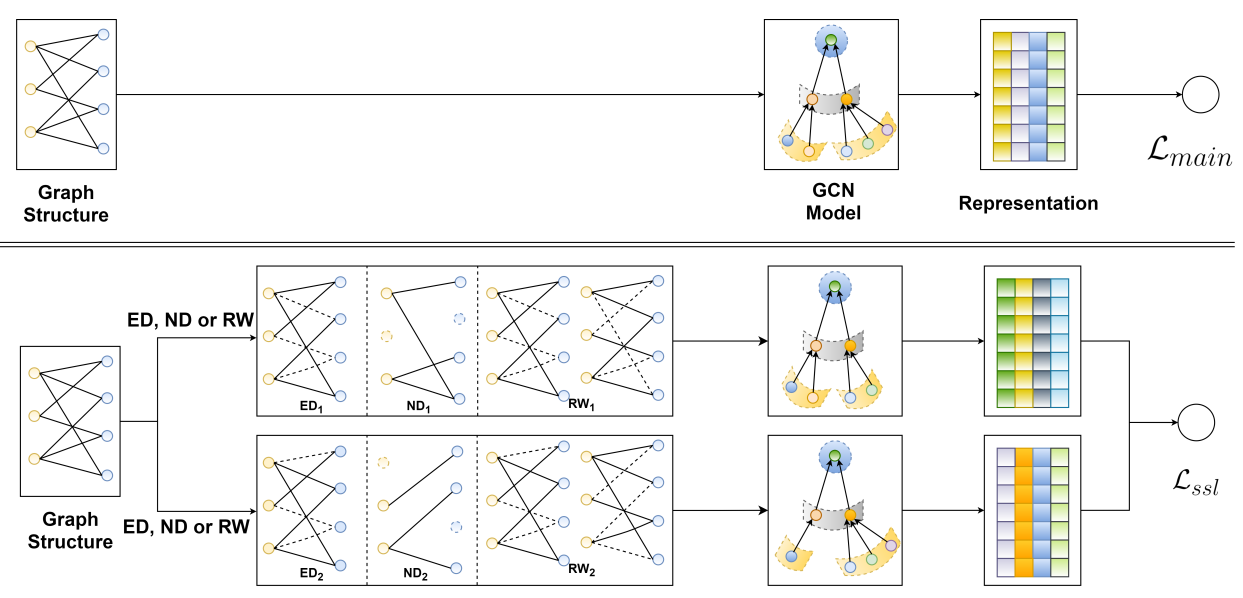
\includegraphics[width=0.9\linewidth]{images/tasks.png}
        \caption{\textbf{Tổng thể hệ thống}. Phía trên minh họa cho task chính học giám sát, phía dưới minh họa cho task học tự giám sát áp dụng các data augmentation trên cấu trúc đồ thị \cite{sgl}}
        \label{fig:tasks}
    \end{figure}
    
    Để cải thiện hệ thống gợi ý (recommendation system), ta áp dụng nó đồng thời với Self-supervised Learning task. Lúc này, recommendation task đóng vai trò chính, self-supervised learning đóng vai trò bổ trợ nhằm tối ưu mô hình gợi ý cổ điển. Đây là \textbf{Joint Learning} (Training Scheme).

    Ta không thể áp dụng các kỹ thuật tăng cường dữ liệu như bài toán Computer Vision (CV) hay Natural Language Processing (NLP) vì các đặc trưng của user, item là rời rạc. Bên cạnh đó, chúng còn được kết nối và phụ thuộc lẫn nhau. Về cấu trúc đồ thị, các nút lân cận bậc nhất là lịch sử người dùng, các nút lân cận bậc hai thể hiện người dùng/hành vi tương tự. Vì vậy ta có thể áp dụng \textbf{Data Augmentation} như bỏ cạnh (edge dropout), bỏ node (node dropout), random walk để tạo ra các “view" khác nhau từ đồ thị gốc ban đầu.

    Với self-supervised learning task trong đề tài này, ta sẽ áp dụng \textbf{contrastive learning}. Với các “view" được tạo ra từ bước Data Augmentation, ta sẽ học được cách biểu diễn, từ đó giúp các “view" khác nhau của cùng một node tiến lại gần nhau, các “view" của các node khác nhau đẩy ra xa nhau.    
    
    \subsection{Kết quả dự kiến của đề tài}
    Bài toán xây dựng hệ thống gợi ý và việc áp dụng kỹ thuật học tự giám sát cho mạng học sâu đồ thị trên bài toán này còn mới và có rất nhiều tiềm năng để phát triển.
    \begin{itemize}
        \item Ở trong phạm vi khóa luận này, nhóm sẽ giải thích được các khái niệm liên quan đến hệ thống gợi ý lẫn học tự giám sát nhằm xây dựng nền tảng vững chắc cho việc phát triển.
        \item Sau khi đã hiểu rõ các kiến thức xung quanh đề tài, nhóm sẽ tiến hành cài đặt thuật toán. Lúc này, ta có thể so sánh kết quả với các bài báo liên quan để so sánh với các mô hình khác, từ đó rút ra nhận xét về mô hình, lẫn ưu nhược điểm. 
        \item Sau cùng mới tiến hành cải tiến nhằm giải quyết các vấn đề còn tồn đọng nếu còn thời gian.

    \end{itemize}
    
    \subsection{Kế hoạch thực hiện}
        
    Phần này mô tả về kế hoạch thực hiện (với các mốc thời gian tương ứng) cùng với việc phân chia công việc cho các thành viên tham gia đề tài.
    \begin{itemize}
        \item Giai đoạn 1 (1/2023 -- 2/2023): Tìm hiểu lý thuyết về học tự giám sát, hệ thống gợi ý và các thuật ngữ/khái niệm xung quanh nó. Cụ thể, sinh viên Hồ Trần Việt Cường sẽ tìm hiểu các kiến thức về bài toán hệ thống gợi ý và các vấn đề mà một hệ thống gợi ý đang gặp phải. Trong khi đó, sinh viên Nguyễn Trung Dũng sẽ tìm hiểu về học tự giám sát và giải thích được vì sao học tự giám sát lại áp dụng được và nếu áp dụng thì sẽ giải quyết được vấn đề gì.
        \item Giai đoạn 2 (3/2023 -- nửa đầu tháng 4/2023): Tìm hiểu các phương pháp/hướng tiếp cận phổ biến mà đã được nghiên cứu/áp dụng trước đó, song song với đó là hệ thống các kiến thức đã tìm hiểu ở giai đoạn trước nhằm chuẩn bị cho việc báo cáo khóa luận tốt nghiệp
        \item Giai đoạn 3 (nửa cuối tháng 4/2023 -- nửa đầu tháng 6/2023): Tiến hành cài đặt và thử nghiệm thuật toán, song song với đó là viết báo cáo khóa luận tốt nghiệp.
        \item Giai đoạn 4 (nửa cuối tháng 6/2023 -- kết thúc): Chỉnh sửa và hoàn thiện báo cáo khóa luận.
    \end{itemize}

    
    \pagebreak 
    %TÀI LIỆU TRÍCH DẪN
    %Đây là ví dụ
    \bibliographystyle{ieeetr}
    \bibliography{sample}
    \nocite{*}

    \begin{table}[h]
    \centering
        \begin{tabular}{p{7cm}p{7cm}}
        \textbf{\begin{tabular}[c]{@{}c@{}}\\XÁC NHẬN\\CỦA NGƯỜI HƯỚNG DẪN\\ \textit{(Ký và ghi rõ họ tên)}\end{tabular}} & \textbf{\begin{tabular}[c]{@{}c@{}}\textit{TP. Hồ Chí Minh, ngày... tháng... năm...}\\NHÓM SINH VIÊN THỰC HIỆN\\\textit{(Ký và ghi rõ họ tên}) \end{tabular}}
        \end{tabular}
    \end{table}
    
\end{document}


